\section{Readout: No Single Scaling Trend}
\label{sec:readout}

The representation--readout gap is the held-out-selected probe accuracy minus the model's own
forced-choice accuracy, at three shots (Figure~\ref{fig:gap}; Table~\ref{tab:gap}).

\begin{figure}[tb]
  \centering
  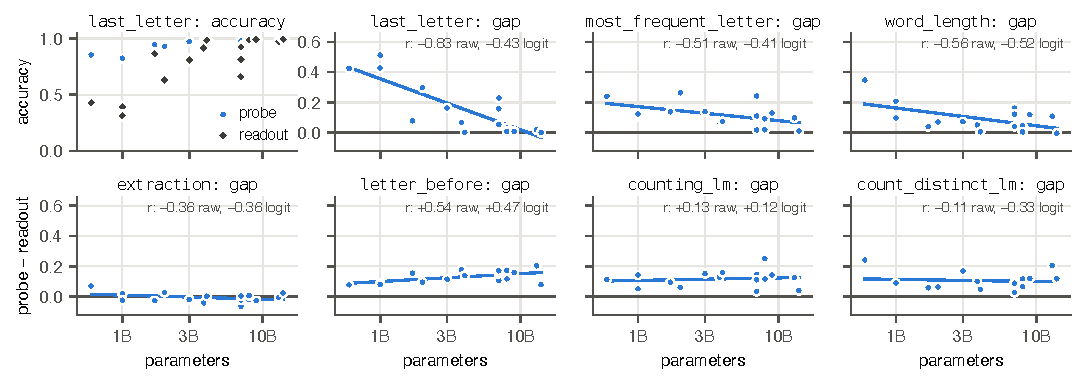
\includegraphics[width=\linewidth]{fig_gap.pdf}
  \caption{Readout at three shots, one point per model. First panel: \texttt{last\_letter} probe
    (held-out-selected) and forced-choice readout accuracy. Other panels: the
    representation--readout gap (probe $-$ readout) with an OLS line, and its correlation with
    $\log_{10}$ parameters on the raw and the logit scale. The correlations are uncorrected for the
    $7 \times 3$ tests; permutation $p$-values, base-only correlations and the mean gap in the three
    smallest and three largest models are in Table~\ref{tab:gap}.}
  \label{fig:gap}
\end{figure}

\paragraph{The \texttt{last\_letter} narrowing is a ceiling effect.}
On the raw scale, \texttt{last\_letter}'s gap falls from $+0.455$ in the smallest models to $+0.009$ in
the largest ($r = -0.83$). In the largest models the probe is at 0.99--1.00 and readout catches up to
it. On the logit scale, which does not compress differences near 1.0, the association is
$r = -0.43$ ($p = 0.09$). Our pre-registered criterion required $|r| \geq 0.4$ \emph{and}
$p < 0.05$ on the logit scale to keep a narrowing claim, so we make none.

\paragraph{Other tasks disagree with one another.}
The gap narrows for \texttt{word\_length} on both scales ($r = -0.52$ on the logit scale,
$p = 0.034$), shows no trend for \texttt{extraction} (where it is near zero at every size), and grows
for \texttt{letter\_before} ($r = +0.54$, $p = 0.033$; base models only, $r = +0.82$). The two
rebuilt count tasks hold a gap of about $+0.10$ to $+0.15$ at every scale. With 21 uncorrected tests,
none of these individually supports a claim. Together they rule out a single scaling trend, and they
do not support the idea that gaps close for retrieval-like tasks and persist for computational ones:
\texttt{extraction} and \texttt{letter\_before} are both retrieval-like and behave oppositely. The probe
also has hundreds of labelled examples while the model sees three demonstrations, so the gap is not
a calibrated measure of unused capacity.

\paragraph{The answer-token subspace.}
At the final layer the output head separates answers only along the span of the answer tokens'
unembedding rows. Projecting the final-layer state onto that span and re-probing beats a random
subspace of the same rank by $+0.12$ (159 of 176 cells, three shots) but beats the top principal
components of the same rank by only $+0.023$. The span is informative, but not much more so than a
label-free comparator; it captures a median 6\% of the between-class-mean energy. The loss from
projection correlates with the readout gap ($r = 0.64$; deficit 0.015, 0.053 and 0.101 across gap
tertiles), but because the projected representation is nested in the full one, this association does
not show that the span causes the gap. Preliminary runs on a different example sample with a peak-over-layers estimator gave
$+0.136$ and $+0.021$.

\paragraph{Post-trained models (exploratory).}
Six of the 16 models are post-trained. At three shots their answer-token span beats the PCA
comparator by more than the base models' does (model-level means, difference $+0.036$, permutation
$p = 0.012$), and they lose less accuracy under projection ($-0.033$, $p = 0.003$); their readout is
also higher (0.60 against 0.51). Size does not explain this, since the post-trained models are
slightly smaller on average, and at zero shots neither difference is significant ($p = 0.15$). This
is consistent with post-training aligning the late representation more closely with the
answer-token readout directions. It is also confounded with model family, because the post-trained
set is exactly the Qwen3 and Phi-4 models, and the test was not planned in advance. We report it as
an observation, not a finding.
